\chapter{数値的に常微分方程式を解く}
\label{numerical-ordinary}
第\ref{first}章で触れたように、世の中にある大半の微分方程式は解析的に解くことができません。そこで登場するのが数値解析です。計算機の力で微分方程式を数値的に解きます。具体的に関数$y(x)$を求めるのであれば、離散的な(飛び飛びの)値$x_i$に対して、各$y_i$を精度良く求めます。この$y_i$を精度良く求めるために、様々な手法が考案されました。それらを紹介します。

本書では数値解析の手法を紹介することに重点を置きます。よって、数値解析にまつわる丸め誤差や桁落ちなどについては触れません。なお、具体的なアルゴリズムの紹介には疑似コードを使います。






\section{オイラー法}
\label{euler-numerical}
オイラー法は最も簡単な数値解析の手法です。問題とする微分方程式を

\begin{eqnarray}
    \frac{\dd y}{\dd x}=f(x,y)
    \label{differential-1}
\end{eqnarray}

\noindent
とします。また、初期条件を

\begin{eqnarray}
    y(x_0)=Y_0
    \label{terms-1}
\end{eqnarray}

\noindent
とします。

$h$を十分小さい定数として、$y(x+h)$をテイラー展開します。

\begin{eqnarray}
    y(x+h)=y(x)+h\frac{\dd}{\dd x}y(x)+\frac{h^2}{2!}\frac{\dd^2}{\dd x^2}y(x)+\dots
\end{eqnarray}

ここで、$h$は十分小さいので$h$の次数が2以上の項を無視します。すると、式\ref{differential-1}より$\dd y(x)/\dd x$を$f(x,y)$に置換して、

\begin{eqnarray}
    y(x+h)=y(x)+hf(x,y(x))
\end{eqnarray}

\noindent
となります。この式は何を意味するでしょうか。右辺は$y(x)$と$x$、および与えられた関数$f$で構成された式、左辺は$y(x+h)$です。そうです。第\ref{first}章で少しお話しした、「今($y(x)$)の状態から少し先の未来($y(x+h)$)を知る」方程式です。図\ref{fig:4-euler}を参照してください。

\begin{figure}[ht!]
  \centering
  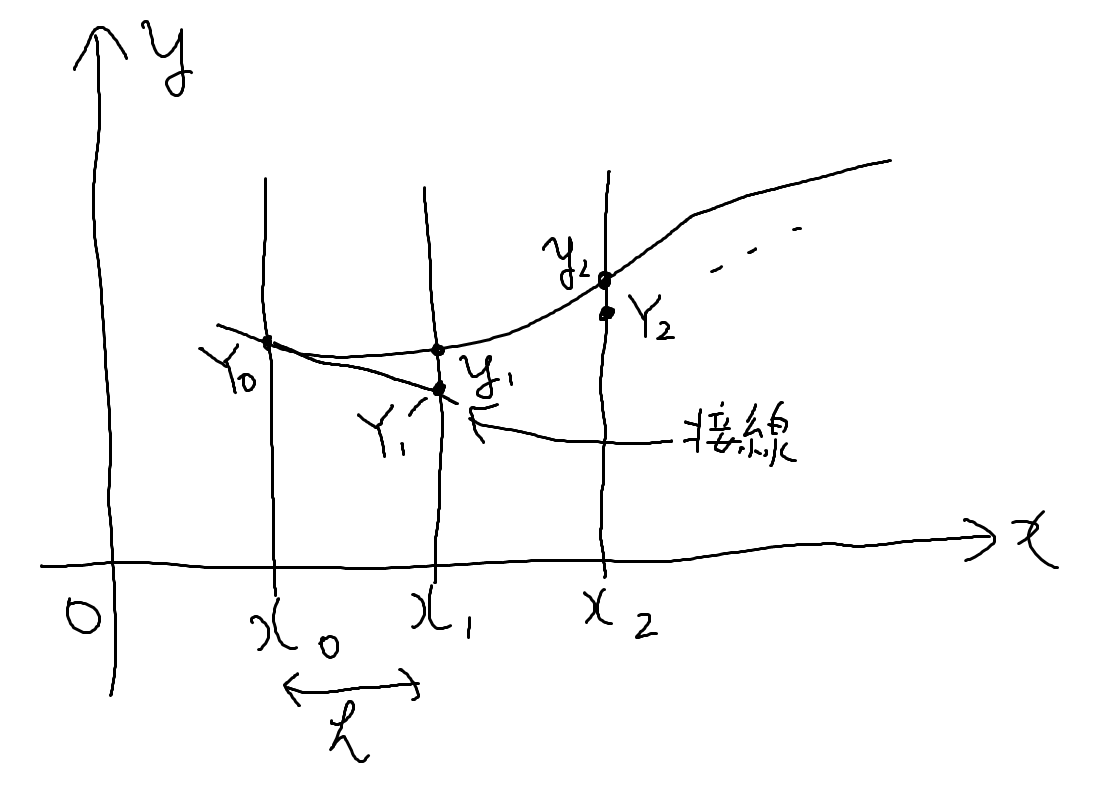
\includegraphics[width=7cm]{img/4-euler.png}
  \caption{オイラー法のイメージ}
  \label{fig:4-euler}
\end{figure}

図\ref{fig:4-euler}のように、$h$ごとに取られた各点$x_i$に対して、それぞれに対応する正しい$y$の値$y_i$、および計算機で計算した近似値$Y_i$を考えます。このとき、$h$を「刻み幅」と言います。刻み幅は一定である必要はありませんが、ここでは一定としておきます。

この考え方を使うと、$Y_{i+1}$は漸化式のように、

\begin{eqnarray}
    Y_{i+1}=Y_i+hf(x_i,Y_i)
\end{eqnarray}

\noindent
と書けます。この式を使って初期条件$x_0$で$Y_0$から順番に$x$を進めていくことで、関数$y$の近似を求めることができます。

擬似コードを以下に示します。

\begin{algorithm}
\caption{オイラー法}
\begin{algorithmic}
\REQUIRE $x_0,Y_0,h,N$
\ENSURE $x_N,Y_N$
\FOR{i=0 \TO N}
    \STATE $x_i\Leftarrow x_0+h\times i$
    \STATE $Y_{i+1}=Y_i+h\times f(x_i,Y_i)$
\ENDFOR
\RETURN $Y_N$
\end{algorithmic}
\end{algorithm}







\section{改良オイラー法}
\label{adv-euler}




\clearpage